\section{QFT, history routing}
11076 hops; seeds 60, 61; every run completed every hop and passed the physical audit (Checks sheet of the workbook).
\subsection{Headline: 8 memories per core, 6 for pre-generation}
ODG, CGP, ACGP and Dynamic~(8) use 8 memories per core, of which 6 may hold pre-generated pairs; Dynamic~($\infty$) uses 64, which no core ever fills.
\begin{table}[H]\centering\small
\begin{tabular}{lrrrrrrr}\toprule
Configuration & Latency (ms) & p95 (ms) & Fidelity & Hop cov. (\%) & Chain full (\%) & Wastage (\%) & Utilisation (\%)\\\midrule
ODG & 1.773 & 4.40 & 0.9498 & 0.0 & 0.0 & -- & --\\
CGP & 0.966 & 3.10 & 0.9422 & 73.8 & 52.6 & 4.97 & 95.0\\
ACGP & 0.917 & 2.95 & 0.9425 & 76.6 & 57.4 & 4.34 & 95.7\\
Dynamic (8) & 0.693 & 2.00 & 0.9442 & 79.6 & 65.7 & 1.40 & 98.6\\
Dynamic ($\infty$) & 0.584 & 1.45 & 0.9450 & 85.6 & 72.4 & 1.46 & 98.5\\
\bottomrule\end{tabular}
\caption{QFT, history routing, 8 memories per core, 6 for pre-generation: mean of the seeds.}\end{table}
\begin{figure}[H]\centering
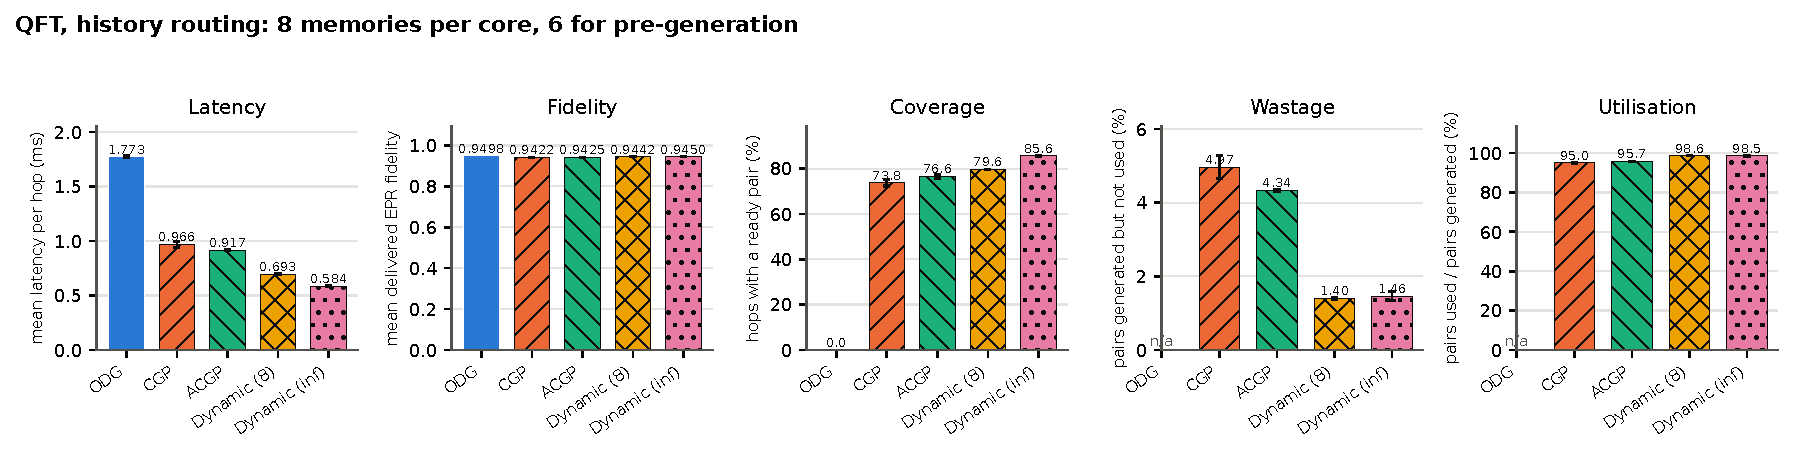
\includegraphics[width=\linewidth]{qft_history_headline_8.pdf}
\caption{QFT, history routing, 8 memories per core, 6 for pre-generation. Bars are the mean of the seeds, whiskers the seed range; fidelity bars start at zero, so read the labels.}\end{figure}
\subsection{Headline: 4 memories per core, all 4 for pre-generation}
ODG, CGP, ACGP and Dynamic~(4) use 4 memories per core and ODG and Dynamic may use all 4 for pre-generation; CGP and ACGP cache at most 3 (all 4 starves them), the same as in the $K$ sweep; Dynamic~($\infty$) as above.
\begin{table}[H]\centering\small
\begin{tabular}{lrrrrrrr}\toprule
Configuration & Latency (ms) & p95 (ms) & Fidelity & Hop cov. (\%) & Chain full (\%) & Wastage (\%) & Utilisation (\%)\\\midrule
ODG & 1.824 & 4.60 & 0.9498 & 0.0 & 0.0 & -- & --\\
CGP & 2.192 & 8.10 & 0.9413 & 63.5 & 40.3 & 5.37 & 94.6\\
ACGP & 2.194 & 8.14 & 0.9412 & 62.3 & 38.3 & 5.44 & 94.6\\
Dynamic (4) & 1.199 & 4.20 & 0.9423 & 65.8 & 55.5 & 4.45 & 95.6\\
Dynamic ($\infty$) & 0.584 & 1.45 & 0.9450 & 85.6 & 72.4 & 1.46 & 98.5\\
\bottomrule\end{tabular}
\caption{QFT, history routing, 4 memories per core, all 4 for pre-generation: mean of the seeds.}\end{table}
\begin{figure}[H]\centering
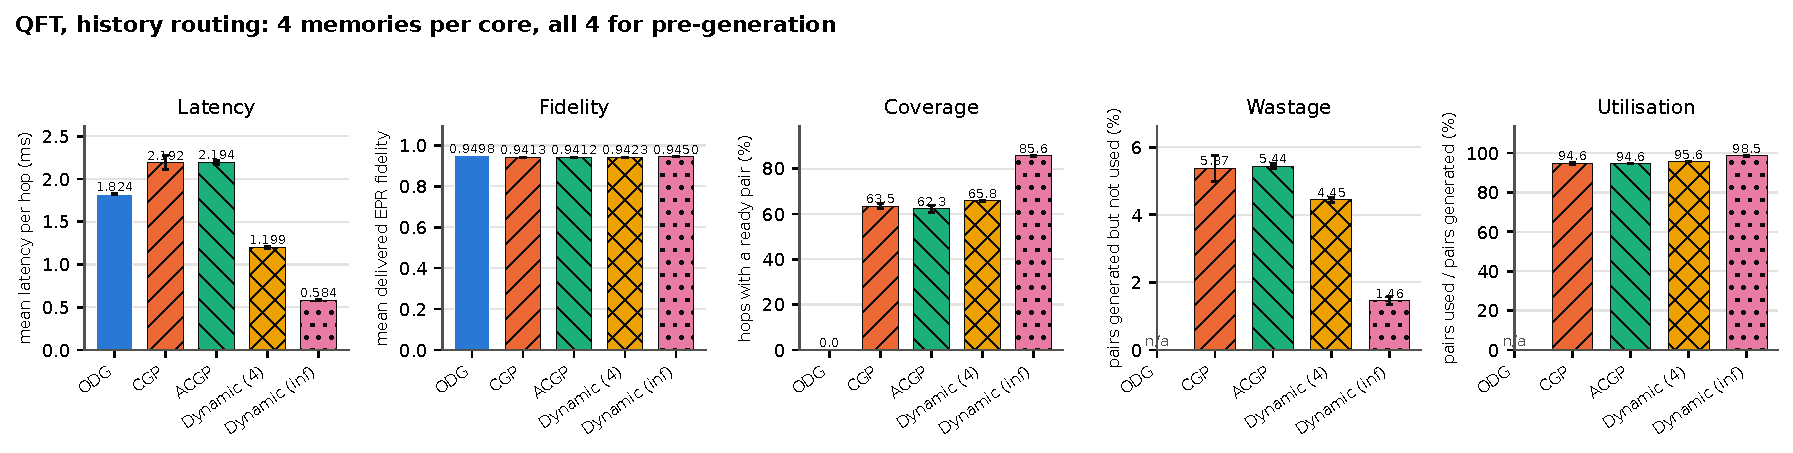
\includegraphics[width=\linewidth]{qft_history_headline_4all.pdf}
\caption{QFT, history routing, 4 memories per core, all 4 for pre-generation. Bars are the mean of the seeds, whiskers the seed range; fidelity bars start at zero, so read the labels.}\end{figure}
\subsection{Memories per core K}
Dynamic may use all K memories, except 6 of 8 at $K=8$; CGP and ACGP cache $\lfloor 0.75K\rfloor$ pairs (so at $K=1$ they are ODG). $K=\infty$ is 64 memories.
\begin{table}[H]\centering\small
\begin{tabular}{lrrrrrrr}\toprule
Latency & $K=1$ & $K=2$ & $K=3$ & $K=4$ & $K=6$ & $K=8$ & $K=\infty$\\\midrule
ODG & 5.820 & 2.554 & 1.963 & 1.824 & 1.776 & 1.773 & 1.773\\
CGP & 5.820 & 3.739 & 2.767 & 2.192 & 1.112 & 0.966 & 0.457\\
ACGP & 5.820 & 3.748 & 2.696 & 2.194 & 1.113 & 0.917 & 0.455\\
Dynamic & 8.812 & 3.153 & 1.749 & 1.199 & 0.797 & 0.693 & 0.584\\
\bottomrule\end{tabular}
\caption{QFT, history routing: latency (mean latency per hop (ms)) for every K.}\end{table}
\begin{figure}[H]\centering
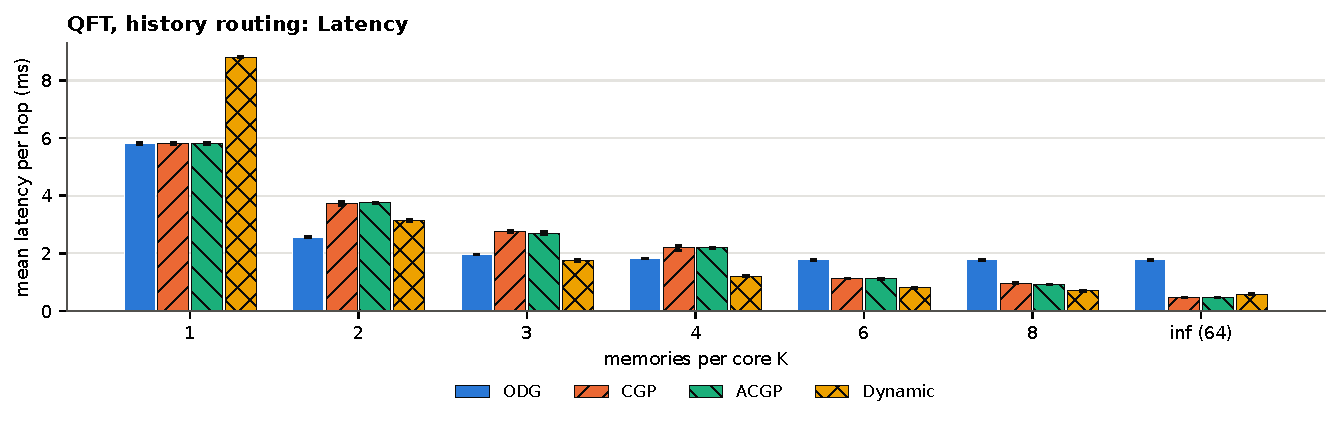
\includegraphics[width=\linewidth]{qft_history_k_latency_ms.pdf}
\caption{QFT, history routing: latency for every K.}\end{figure}
\begin{table}[H]\centering\small
\begin{tabular}{lrrrrrrr}\toprule
Fidelity & $K=1$ & $K=2$ & $K=3$ & $K=4$ & $K=6$ & $K=8$ & $K=\infty$\\\midrule
ODG & 0.9498 & 0.9498 & 0.9498 & 0.9498 & 0.9498 & 0.9498 & 0.9498\\
CGP & 0.9498 & 0.9452 & 0.9427 & 0.9413 & 0.9433 & 0.9422 & 0.9417\\
ACGP & 0.9498 & 0.9449 & 0.9426 & 0.9412 & 0.9433 & 0.9425 & 0.9418\\
Dynamic & 0.9487 & 0.9442 & 0.9427 & 0.9423 & 0.9439 & 0.9442 & 0.9450\\
\bottomrule\end{tabular}
\caption{QFT, history routing: fidelity (mean delivered EPR fidelity) for every K.}\end{table}
\begin{figure}[H]\centering
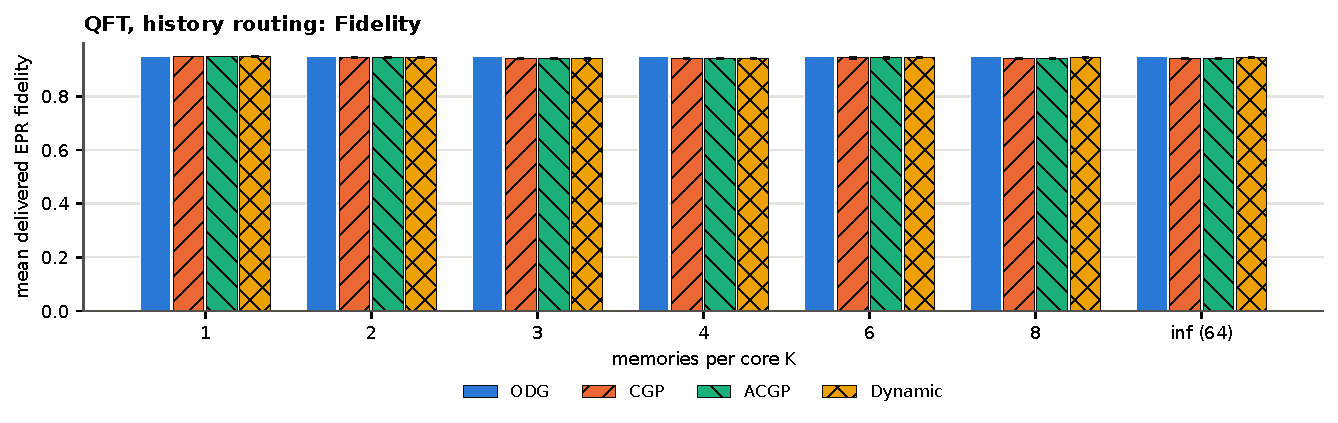
\includegraphics[width=\linewidth]{qft_history_k_fidelity.pdf}
\caption{QFT, history routing: fidelity for every K.}\end{figure}
\begin{table}[H]\centering\small
\begin{tabular}{lrrrrrrr}\toprule
Coverage & $K=1$ & $K=2$ & $K=3$ & $K=4$ & $K=6$ & $K=8$ & $K=\infty$\\\midrule
ODG & 0.0 & 0.0 & 0.0 & 0.0 & 0.0 & 0.0 & 0.0\\
CGP & 0.0 & 27.2 & 47.8 & 63.5 & 64.2 & 73.8 & 99.2\\
ACGP & 0.0 & 28.2 & 49.7 & 62.3 & 65.3 & 76.6 & 99.5\\
Dynamic & 8.4 & 36.4 & 53.8 & 65.8 & 79.2 & 79.6 & 85.6\\
\bottomrule\end{tabular}
\caption{QFT, history routing: coverage (hops with a ready pair (\%)) for every K.}\end{table}
\begin{figure}[H]\centering
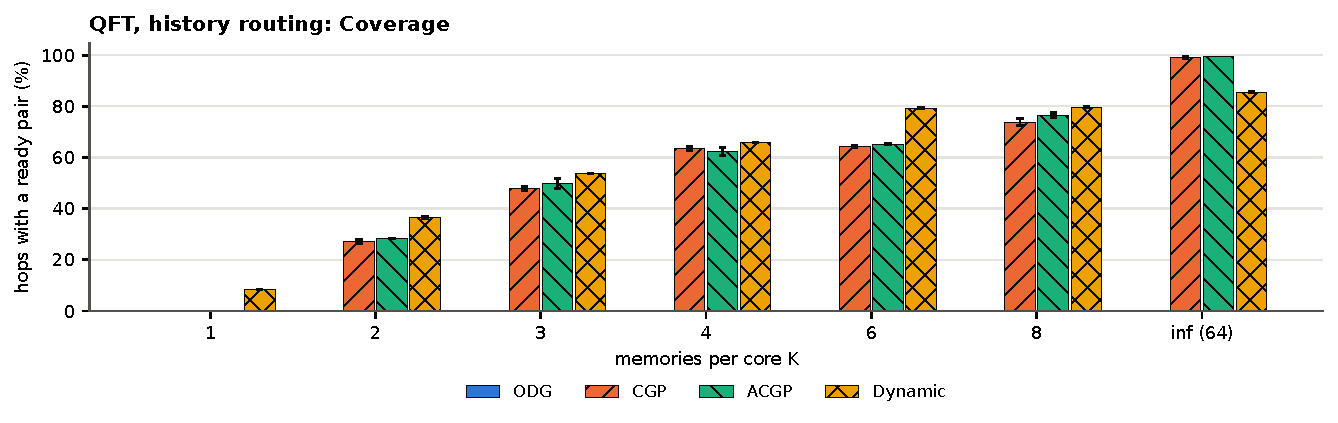
\includegraphics[width=\linewidth]{qft_history_k_hop_coverage_pct.pdf}
\caption{QFT, history routing: coverage for every K.}\end{figure}
\begin{table}[H]\centering\small
\begin{tabular}{lrrrrrrr}\toprule
Wastage & $K=1$ & $K=2$ & $K=3$ & $K=4$ & $K=6$ & $K=8$ & $K=\infty$\\\midrule
ODG & -- & -- & -- & -- & -- & -- & --\\
CGP & -- & 6.23 & 5.85 & 5.37 & 3.96 & 4.97 & 14.14\\
ACGP & -- & 6.07 & 5.58 & 5.44 & 3.74 & 4.34 & 13.66\\
Dynamic & 63.26 & 14.98 & 6.07 & 4.45 & 2.25 & 1.40 & 1.46\\
\bottomrule\end{tabular}
\caption{QFT, history routing: wastage (pairs generated but not used (\%)) for every K.}\end{table}
\begin{figure}[H]\centering
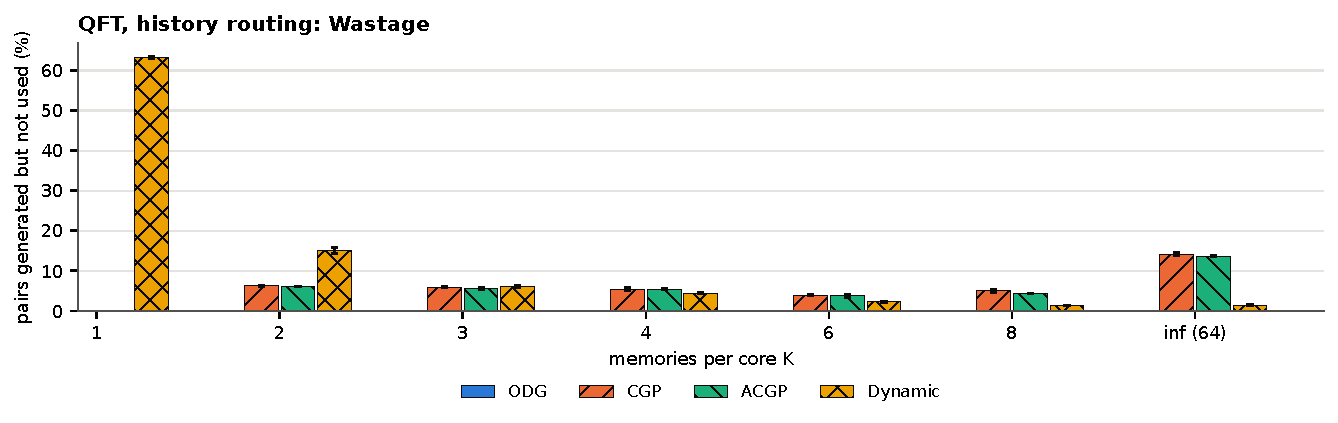
\includegraphics[width=\linewidth]{qft_history_k_wastage_pct.pdf}
\caption{QFT, history routing: wastage for every K.}\end{figure}
\begin{table}[H]\centering\small
\begin{tabular}{lrrrrrrr}\toprule
Utilisation & $K=1$ & $K=2$ & $K=3$ & $K=4$ & $K=6$ & $K=8$ & $K=\infty$\\\midrule
ODG & -- & -- & -- & -- & -- & -- & --\\
CGP & -- & 93.8 & 94.1 & 94.6 & 96.0 & 95.0 & 85.9\\
ACGP & -- & 93.9 & 94.4 & 94.6 & 96.3 & 95.7 & 86.3\\
Dynamic & 36.7 & 85.0 & 93.9 & 95.6 & 97.7 & 98.6 & 98.5\\
\bottomrule\end{tabular}
\caption{QFT, history routing: utilisation (pairs used / pairs generated (\%)) for every K.}\end{table}
\begin{figure}[H]\centering
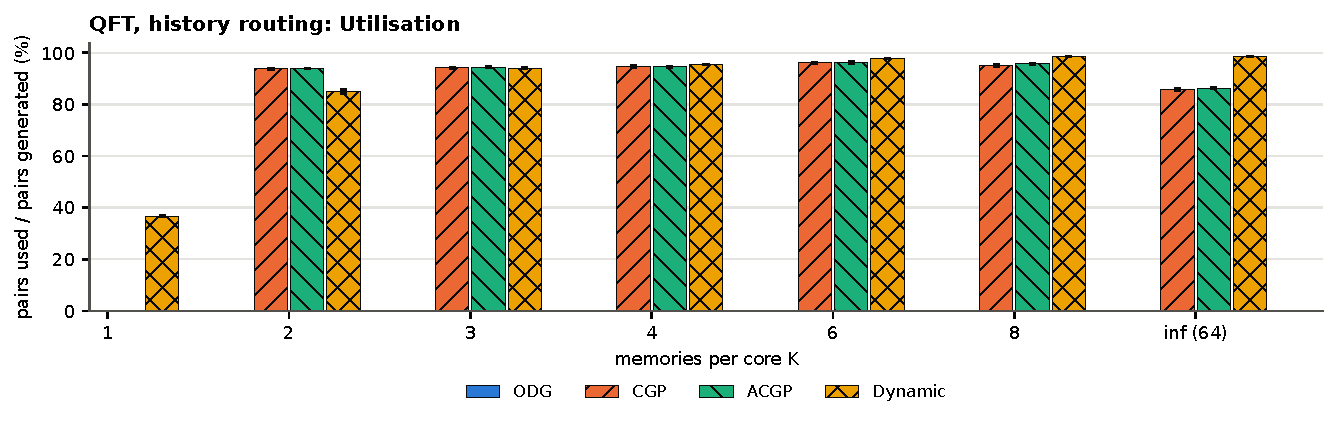
\includegraphics[width=\linewidth]{qft_history_k_utilisation_pct.pdf}
\caption{QFT, history routing: utilisation for every K.}\end{figure}
